\documentclass{report}

\setlength{\textwidth}{150mm}
%\setlength{\textheight}{195mm}
\setlength{\oddsidemargin}{9mm}
%\setlength{\evensidemargin}{28mm}
%\setlength{\topmargin}{-10mm}


\usepackage[utf8]{inputenc}
\usepackage{graphicx}
\graphicspath{ {images/} }
\usepackage{caption}
\usepackage{subcaption}
\usepackage{wrapfig}
\usepackage{listings}
\usepackage[spanish]{babel}
\begin{document}
\begin{titlepage}
\centering

\begin{figure}[t]

\includegraphics[scale=0.5]{images/urjc_logo.png}
\centering
\vspace{0.5cm} %Espacios despúes de la imagen
\end{figure}

{\scshape\Large Escuela Técnica Superior de Ingeniería de Telecomunicación \par}
\vspace{1cm}
{\scshape\Large Grado en Ingeniería en Sistemas de Telecomunicación \par}
\vspace{3cm}
{\bfseries\LARGE INTEGRACIÓN DE ROBOTS FÍSICOS EN LA PLATAFORMA KIBOTICS \par}
\vspace{3cm}
{\itshape\Large Trabajo Fin de Grado \par}
\vfill
{\Large Autor: }
{\Large David ValladaresVigara \par}
{\Large Tutores: }
{\Large Jose María Cañas Plaza y Julio Manuel Vega Pérez \par}
\vfill
{\Large Curso Académico 2019/2020 \par}
\end{titlepage} 

\renewcommand{\abstractname}{\Large Resumen}
\begin{abstract}



\end{abstract}

\setcounter{tocdepth}{3} %Para que aparezcan las subsubsection{}
\renewcommand{\contentsname}{Índice general}
\tableofcontents
\clearpage

\renewcommand{\listfigurename}{Índice de figuras}
\listoffigures

\renewcommand{\listtablename}{Índice de tablas}
\listoftables

\renewcommand{\lstlistingname}{Fragmento}

\renewcommand{\chaptername}{Capítulo}
\chapter{Introducción}

En este capítulo se introducen las aplicaciones de la robótica para el ambiente educativo y las motivaciones que han llevado al desarrollo del Trabajo de Fin de Grado (TFG). Este TFG se ha desarrollado dentro de la plataforma Kibotics para tratar de mejorar la integración sobre robots reales.

\section{Robótica educativa}

La robótica es la ciencia que estudia el diseño y la construcción de máquinas que permiten realizar y facilitar tareas desempeñadas por el ser humano (Quiroga, 2018). Actualmente puede considerarse una de las áreas de las Tecnologías de la Información y Comunicación (TIC) con más auge, pues cada vez es más habitual el uso de robots limpiadores (p. ej. Roomba de iRobot) (Figura 1.1), asistentes virtuales (p. ej. Alexa de Amazon) o el empleo de brazos robóticos en las cadenas de montaje de las industrias. Por ello, resultan muy beneficiosos en el sector industrial y el de servicios (Salamanca, Barrera y Pérez, 2010).
\\
\begin{figure}
  \centering
    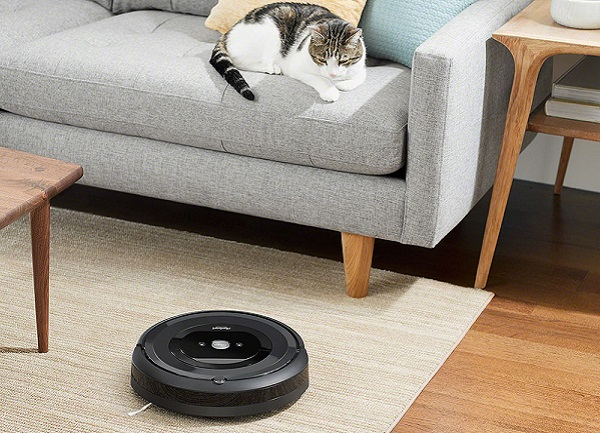
\includegraphics[width=0.4\textwidth]{images/romba.png}
  \caption{Robot aspirador modelo Roomba®}
  \label{Roomba}
\end{figure}
\\

Sin embargo, desde los años sesenta aumentó el interés por introducir la robótica también en el ámbito educativo, creando así la “Robótica educativa” o “Robótica pedagógica”. Se define como una disciplina que permite concebir, diseñar y desarrollar robots educativos para que las personas se puedan iniciar pronto en el mundo de la ciencia y tecnología (Ruiz-Velasco, García y Rosas, 2007). Al combinar diferentes áreas del conocimiento, se ha convertido en una herramienta novedosa que puede utilizarse en las primeras etapas de la educación de los niños y niñas ayudando a potenciar su desarrollo integral (Quiroga, 2018) y que, además, permite que los estudiantes adquieran otras competencias, como la socialización, la creatividad,  la iniciativa y el pensamiento lógico (Bravo y Forero, 2012).
\\

Los orígenes de la robótica educativa se remontan al siglo XX con la teoría constructivista de Jean Piaget, la cual indica que el conocimiento se construye activamente en la mente del estudiante. Esto coincide con la pedagogía del construccionismo de Seymour Papert donde, además, se afirma que lo que construye el individuo debe ser tangible y con un significado personal para él. Algunos desarrollos de la robótica educativa se basan en esta última (González y Jiménez, 2009).
\\

La robótica educativa, por tanto, se considera una herramienta paralela a las asignaturas tradicionales al volverlas más atractivas e integradoras para los estudiantes (Quiroga, 2018). Con ello, ayuda a los alumnos a construir conceptos y a hacer una interpretación personal de la realidad (Salamanca, Barrera y Pérez, 2010).
\\

\subsection{Ejemplo de Metodología para la enseñanza}

Una de las metodologías para llevar a cabo un proceso de trabajo de robótica es la de las cuatro palabras de Báez et al. (2011), representadas en la Figura 1.2. La primera de ellas es “imaginar” porque los estudiantes piensan y debaten sobre dispositivos que pueden ser útiles para resolver un problema o facilitar un trabajo, lo que favorece al pensamiento creativo. A continuación, encontramos la palabra “diseñar”, que les permite crear el artefacto que han imaginado consiguiendo una conexión entre el mundo físico y la imaginación. La tercera es “construir”, que se basa en el montaje de los dispositivos que han diseñado los miembros del grupo de trabajo, por lo que favorece la cooperación y el trabajo manual. La última palabra del proceso es “programar” o dotar de inteligencia a los dispositivos montados a través de un ordenador, mejorando el pensamiento lógico, la autopercepción y el análisis espacial.
\\
\begin{figure}[h!]
  \centering
    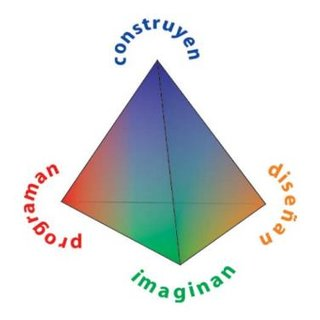
\includegraphics[width=0.4\textwidth]{images/metodologia.png}
  \caption{Las cuatro palabras de la Robótica educativa (Báez et al., 2011).}
  \label{Metodologia}
\end{figure}
\\

\subsection{Aumento de la implantación de la robótica en las aulas}

En la última década, la robótica ha adquirido mucha importancia en un gran número de países (Quiroga, 2018), y cada vez genera más interés implantarla en las aulas (Salamanca, Barrera y Pérez, 2010).
\\

Esto se debe a que aporta muchos beneficios en el proceso de enseñanza-aprendizaje de asignaturas difíciles (Moreno et al., 2012). También es más frecuente la creación de robots para la vida cotidiana, lo que despierta el interés de las personas en ellos (Quiroga, 2018). Además, la existencia de lenguajes de programación orientados a alumnos de menor edad (p. ej. Scratch - Figura 1.3) y la mayor disponibilidad de kits de robótica educativa en el mercado los ha convertido en productos ideales para la iniciación en este campo.
\\
\begin{figure}[h!]
  \centering
    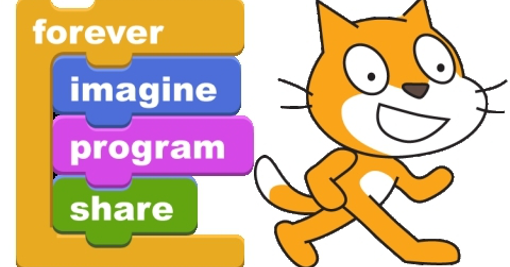
\includegraphics[width=0.3\textwidth]{images/logo_scratch.png}
  \caption{Scratch}
  \label{Scratch}
\end{figure}
\\

Algunos de los robots existentes en el mercado orientados a ese aprendizaje en la robótica son:
\begin{itemize}
	\item \textbf{Mbot}. Diseñado por la empresa MakeBlock y basado en Arduino Uno, una placa electrónica que contiene un microcontrolador programable.
		\begin{figure}[h!]
  			\centering
   			 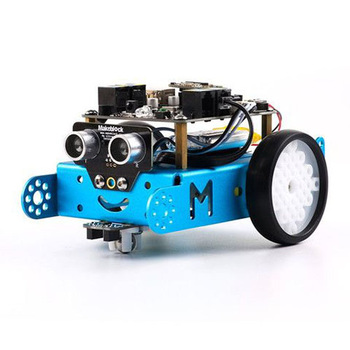
\includegraphics[width=0.3\textwidth]{images/mbot.png}
 			 \caption{Mbot}
 			 \label{Mbot}
		\end{figure}
	\item \textbf{Tello de Ryze Dji }. Es un pequeño dron pensado para que los niños y adultos aprendan su manejo de forma sencilla.
		\begin{figure}[h!]
  			\centering
   			 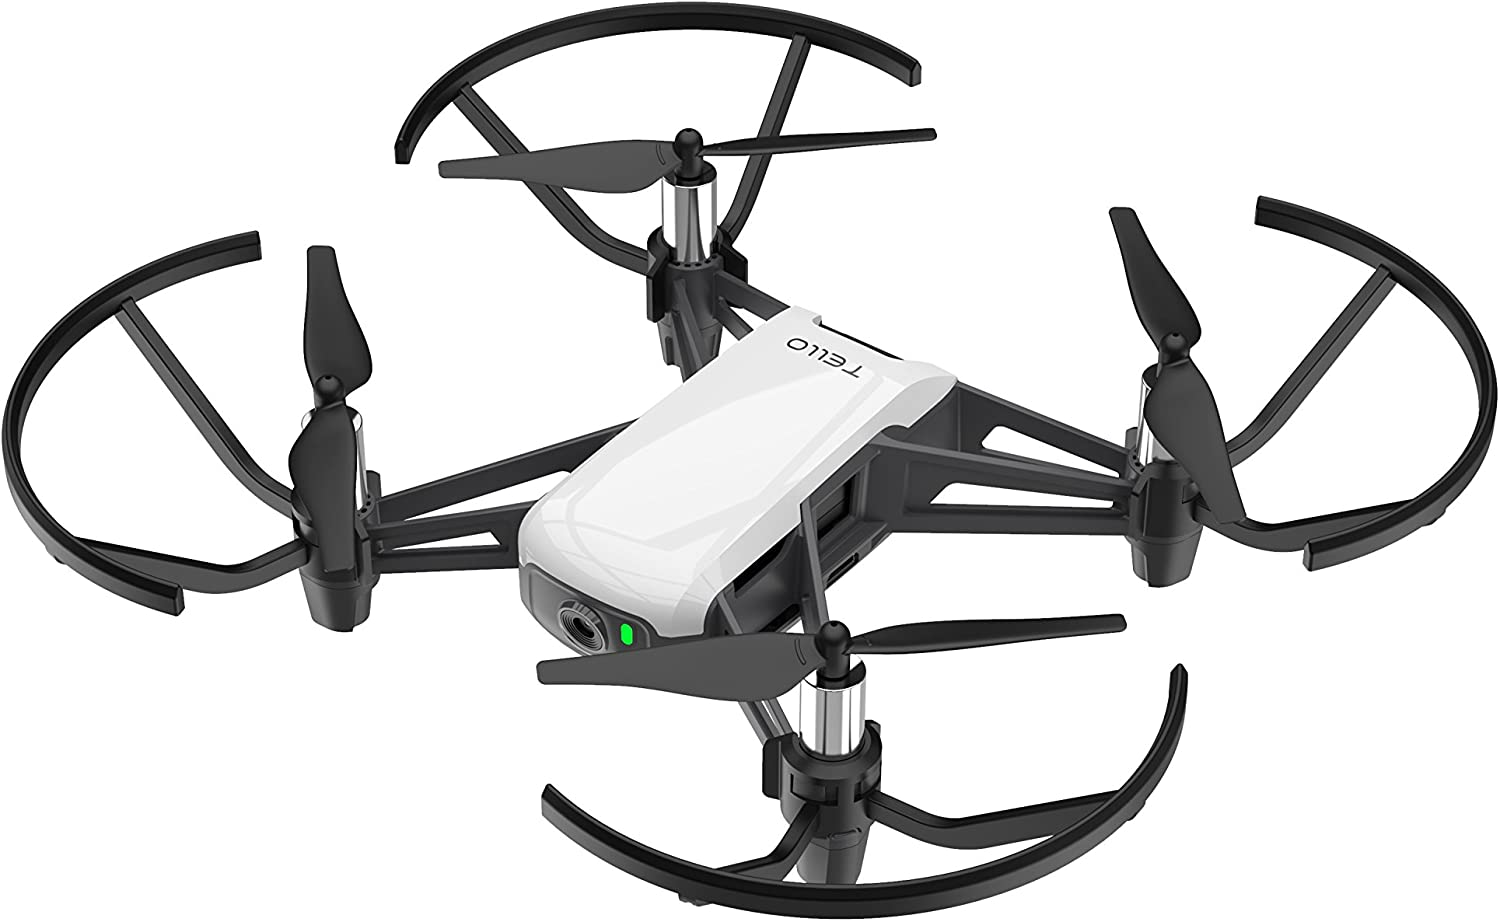
\includegraphics[width=0.3\textwidth]{images/tello.png}
 			 \caption{Tello}
 			 \label{Tello}
		\end{figure}
	\item \textbf{GopiGo3}. Es un robot con forma de coche creado por Dexter Industries, se caracteriza porque su controladora es una RaspberryPi 3, un mini-ordenador de bajo conste que le dota de una gran inteligencia.
		\begin{figure}[h!]
  			\centering
   			 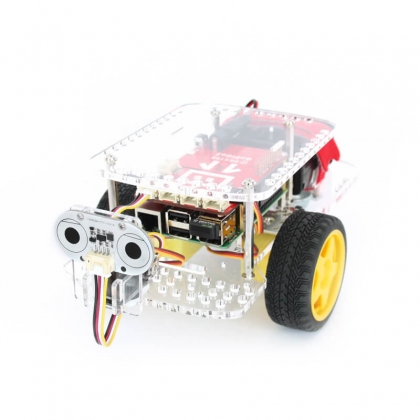
\includegraphics[width=0.3\textwidth]{images/gopigo.png}
 			 \caption{GopiGo3}
 			 \label{GopiGo3}
		\end{figure}
\end{itemize}

Por último, existen aplicaciones y páginas web de programación robótica que facilitan la creación de programas para los robots, como pueden ser Mblock (desarrollada por la empresa MakeBlock y basada en Scratch 3), Bitbloq (creada por la empresa bq, que utiliza bloques para realizar los programas y es compatible con la placa arduino) o Kibotics (llevada a cabo por JdeRobot).
\\

\section{Kibotics}

Kibotics (Figura 1.7) es un entorno web utilizado para la docencia en los campos de robótica, programación y áreas STEM (acrónimo de Science, Technology, Engineering and Mathematics).
\\
\begin{figure}[h!]
  \centering
    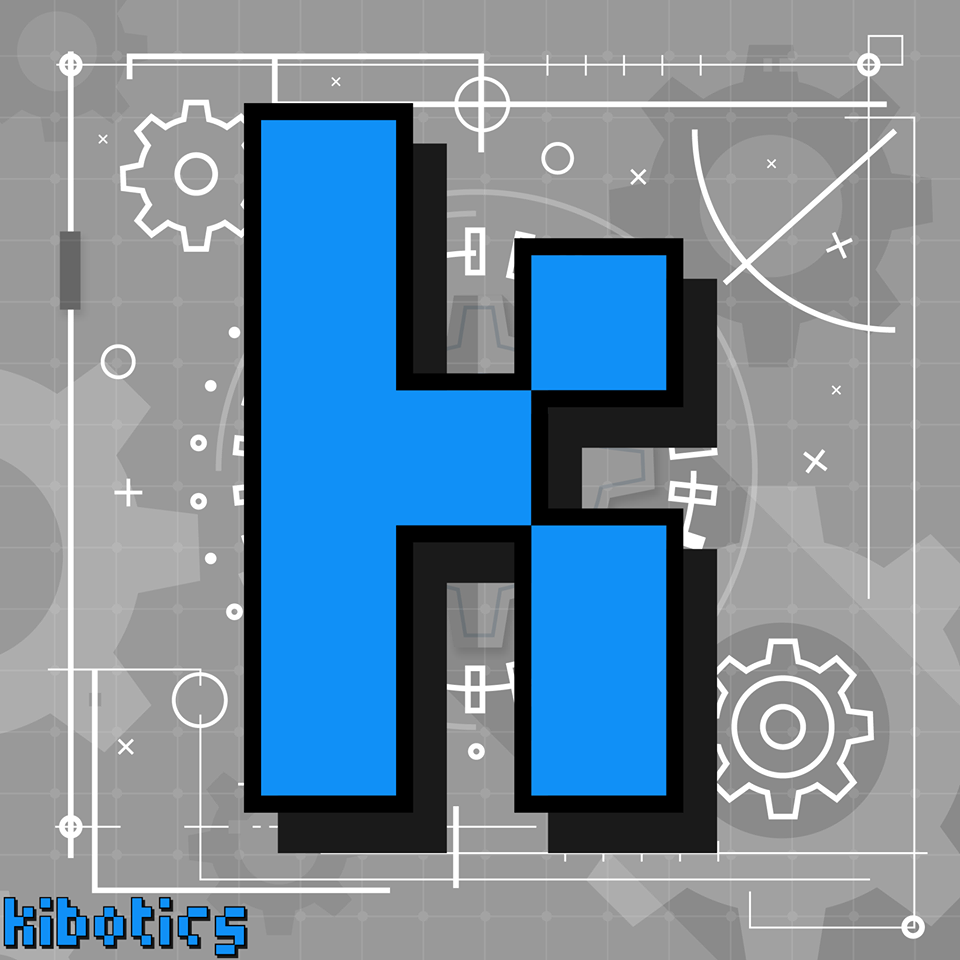
\includegraphics[width=0.3\textwidth]{images/logo_kibotics.png}
  \caption{Logo de Kibotics}
  \label{Logo de Kibotics}
\end{figure}
\\


Ayuda a los alumnos a iniciarse en el mundo de la robótica y la programación de forma sencilla y práctica.
\\

\subsection{Lenguajes soportados en Kibotics}

La plataforma proporciona, actualmente, ejercicios para dos lenguajes de programación. El primero de ellos es Blockly, que fue desarrollado por Google y es muy similar a Scratch. Está orientado para alumnos de menor edad por ser un lenguaje de programación visual basado en una interfaz de bloques que se pueden encajar como si fuera un puzle. Su uso en colegios e institutos es cada vez mayor, ya que está diseñado para que la iniciación al mundo de la programación sea sencilla, divertida y creativa.
\\

Los procedimientos utilizados en la programación de Blockly en Kibotics se clasifican en:
\begin{itemize}
	\item \textit{Serie} : ordenación de los bloques creando una secuencia lógica.

	\item \textit{Bucles}: proporcionan la posibilidad de introducir repeticiones sobre una secuencia deseada.
		
	\item \textit{Variables}: aquellas estructuras de datos en las que se pueden almacenar información a lo largo de la ejecución de un programa.
	
	\item \textit{Operadores lógicos}: devuelve un resultado de verdadero o falso en función de si se cumple o no una determinada condición.
	
	\item \textit{Bloques condicionales}: permiten decidir qué camino lógico tomar en base a una operación lógica.
	
	\item \textit{Operador matemático}: aquellos bloques que permiten realizar una operación matemática.
	
	\item \textit{Robot Api}: se proporciona una interfaz con los actuadores y sensores disponibles para un determinado robot, facilitando así su programación.
\end{itemize}

El segundo es Python, enfocado para alumnos mayores. Constituye uno de los lenguajes de programación con más popularidad en la actualidad según el Índice de Popularidad de Lenguajes de Programación (PYPL PopularitY of Programming Language index, 2020). Es multiparadigma, multiplataforma, gratuito, posee un tipado dinámico e interpretado, es decir, no necesita que un compilador lo procese. Estas características, además de tener una sintaxis legible, permiten un aprendizaje más sencillo que con otros lenguajes de programación como Blockly (Figura 1.8).
\\
\begin{figure}[h!]
  \centering
    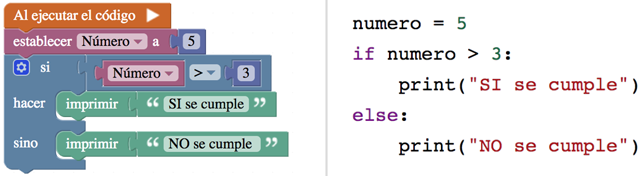
\includegraphics[width=1\textwidth]{images/blockly-vs-python.png}
  \caption{Comparación del mismo código escrito en Blockly (izquierda) y Python (derecha)}
  \label{Comparación del mismo código escrito en Blockly y Python}
\end{figure}
\\

En Kibotics se proporciona una variedad de ejercicios para poner en práctica la programación en Python en diferentes robots. Además, para facilitar el manejo con ellos, se han desarrollado librerías que proporcionan funciones para interactuar con los actuadores y sensores de los robots disponibles. Por ejemplo, en la Figura 1.9 se indican algunas funciones disponibles para el manejo del Dron “Tello”.
\\
\begin{figure}[h!]
  \centering
    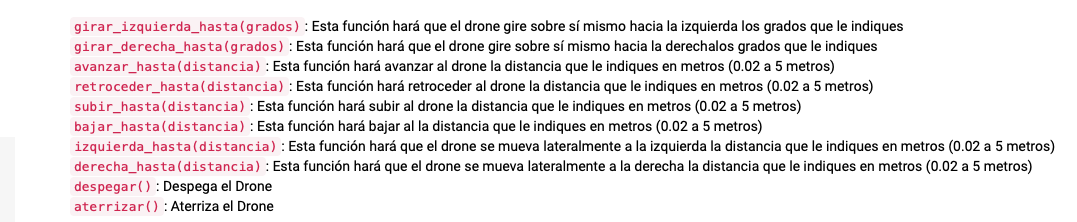
\includegraphics[width=1.1\textwidth]{images/api.png}
  \caption{Funciones disponibles para el Dron “Tello”.}
  \label{Funciones disponibles para el Dron “Tello”.}
\end{figure}
\\

\subsection{Tipos de Robots}

No existe una definición única universal para la palabra “robot”. Por ejemplo, la Real Academia Española (RAE) determina que es una “máquina o ingenio electrónico programable, capaz de manipular objetos y realizar operaciones antes reservadas solo a las personas” (RAE, 2020). También se define como un “sistema compuesto por mecanismos que le permiten hacer movimientos y realizar tareas específicas, programables y eventualmente inteligentes, valiéndose de conceptos de otras áreas del conocimiento” (Salamanca, Barrera y Pérez, 2010).
\\

Un robot se compone, principalmente, de las siguientes partes:
\begin{itemize}
	\item \textit{Esqueleto}. Encargado de soportar los componentes que forman al robot.

	\item \textit{Controladora}. Encargada de procesar los datos obtenidos de los sensores, tomar decisiones y enviar las órdenes a los actuadores.
		
	\item \textit{Sensores o receptores}. Miden magnitudes físicas y las transforman a magnitudes eléctricas. Existen dos tipos, por un lado, están los encargados del entorno que les rodea y, por otro, los del estado interno. Ejemplos de sensores son los infrarrojos, de proximidad, ultrasonido, etc.
	
	\item \textit{Actuadores}. Encargados del movimiento del robot mediante las órdenes recibidas de la controladora.
\end{itemize}

En Kibotics se distinguen dos tipos de robots con los que se puede interactuar: los robots simulados (p. ej. Drone Tello, Mbot, Pibot) y los robots físicos o reales (p. ej. Pibot).
\\

Los robots simulados son robots virtuales que emulan el comportamiento de un robot real, permitiendo al usuario interactuar con él como si fuera uno real (Figura 1.10). Esto se fundamenta en la idea de Robert E. Shannon de simulación como “un proceso de diseñar un modelo de un sistema real y llevar a termino experiencias con él, con la finalidad de comprender el comportamiento del sistema o evaluar nuevas estrategias para el funcionamiento del sistema” (Shannon, 1998).  Al trabajar con ellos, no se necesita su presencia física, se crea una interacción más segura y se puede experimentar con situaciones más complejas o con las que no se posee información.
\\
\begin{figure}[h!]
  \centering
    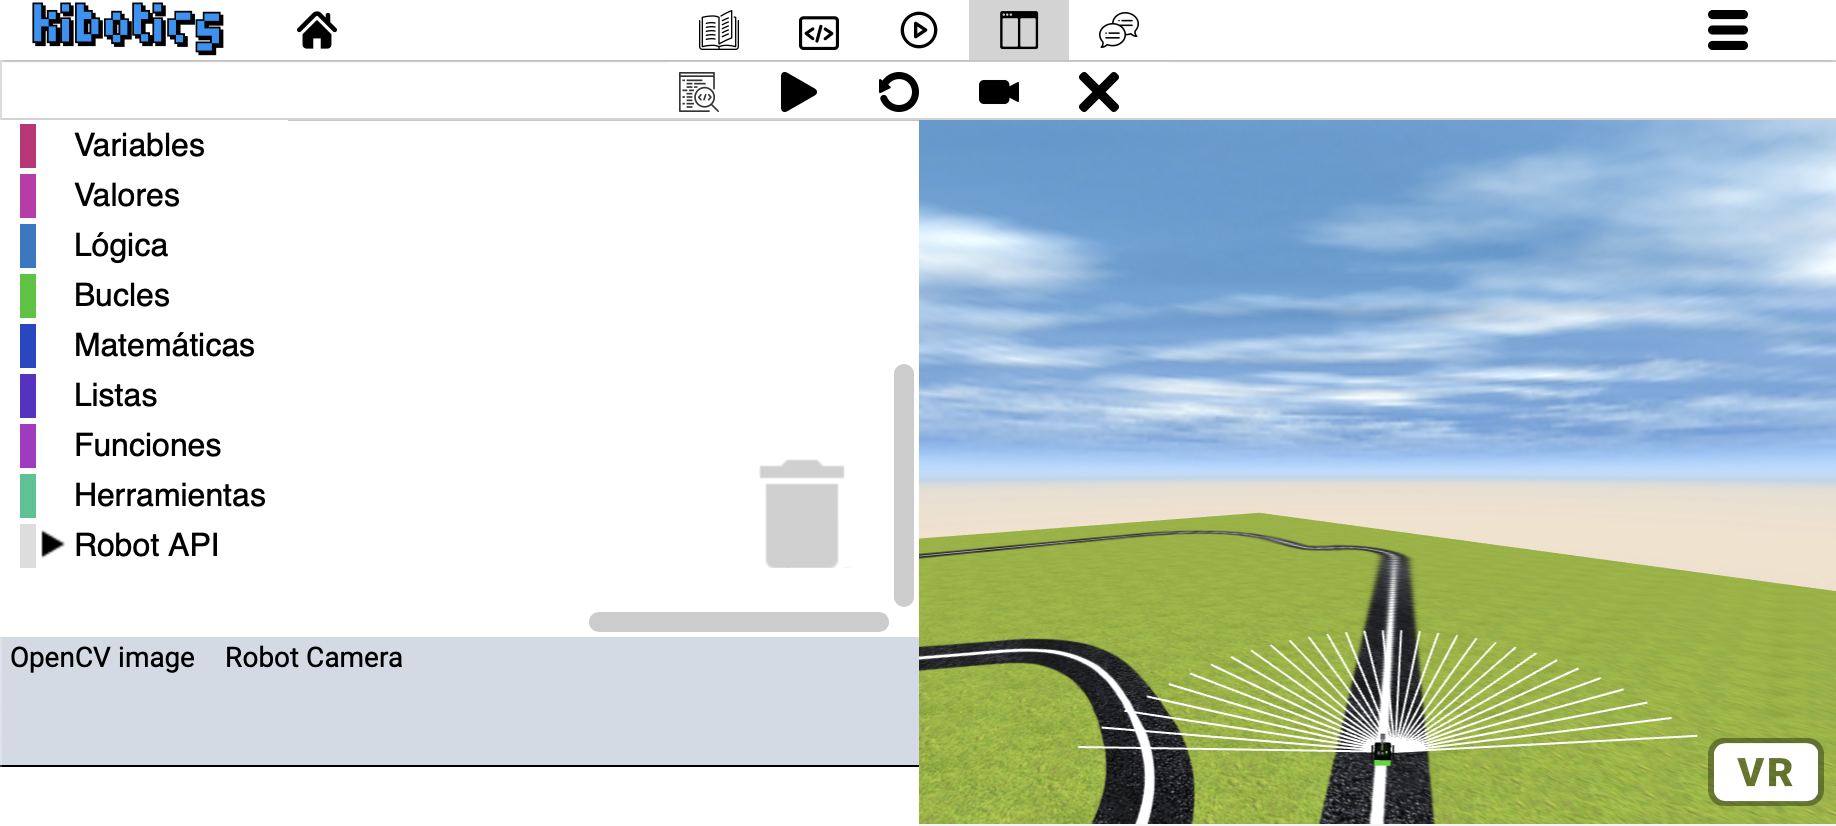
\includegraphics[width=0.9\textwidth]{images/simulado.png}
  \caption{Ejemplo de Robot simulado en Kibotics}
  \label{Ejemplo de Robot simulado en Kibotics}
\end{figure}
\\

En cuanto a los robots físicos o reales, desde Kibotics se da soporte para el desarrollo de programas y envíos sobre algunos de ellos, por ejemplo, para el Pibot mencionado anteriormente. Con ello, se pretende facilitar este proceso de comunicación, que en muchas ocasiones puede no ser sencillo.
\\

En este punto recae la motivación principal para este TFG, que consiste en proporcionar soporte para el uso sobre robots reales, como Mbot, Tello y Gopgio, aunque se hablará más en detalle en el capítulo dos.

\chapter{Objetivos}

\section{Objetivos}
\section{Metodología}
\section{Requerimientos}

\chapter{Herramientas}

\chapter{Integracion Mbot en Kibotics}
En este capítulo se aborda el proceso de integración que va a permitir programar al robot físico Mbot sin necesidad de una instalación previa ni descargas adicionales.

\section{Características del Mbot}

Mbot es un robot fácil de montar y con una estructura robusta, orientado para empezar el aprendizaje de la robótica y la programación desde la educación primaria. Está diseñado por la empresa MakeBlock, la cual dispone de una gran variedad de recursos, robots y kits de robotica.
El robot pesa 400 gramos y sus dimensiones son de 17x13x9 cm. Respecto a las especificaciones técnicas, posee una placa llamada “mCore” que está basada en ArduinoUno, dispone de una microcontroladora ATmega238, cuatro puertos Rj25, un interruptor de encendido, dos leds RGB, un botón, zumbador, un sensor de infrarrojos y otro de luminosidad. Dispone de una batería de litio de 3,7V, pero también funciona con cuatro pilas de tipo AA. En cuanto  sus módulos externos, presenta dos motes, ultrasonido y un seguidor en línea, aunque también pueden utilizarse otras conexiones adicionales. Se comunica por vía puerto serie o por Bluetooth 4.0 (Robótica Educativa con Mbot, 2020).
\\
\begin{figure}[h!]
  \centering
    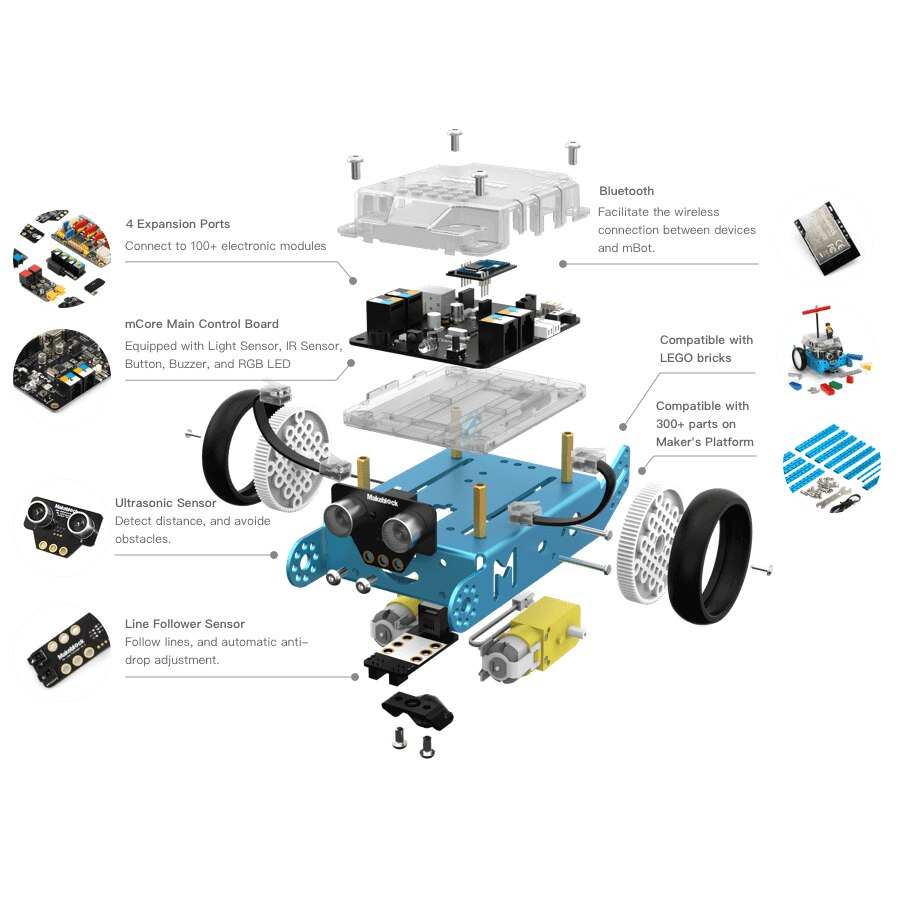
\includegraphics[width=0.9\textwidth]{images/partes_mbot.png}
  \caption{Partes robot Mbot}
  \label{figura:Partes robot Mbot}
\end{figure}
\\
\section{Proceso de envío desde la plataforma Kibotics}

Desde la parrilla principal de Kibotics se puede entrar a la unidad dedicada al Mbot, pudiendo elegir qué lenguaje de programación usar (Python o Blockly). Dentro de dicha unidad encontramos un apartado dedicado a proporcionar las instrucciones necesarias para realizar un programa y enviárselo al Mbot y otro donde se proporciona el editor que permite escribir el programa.
\\
\begin{figure}[h!]
  \centering
    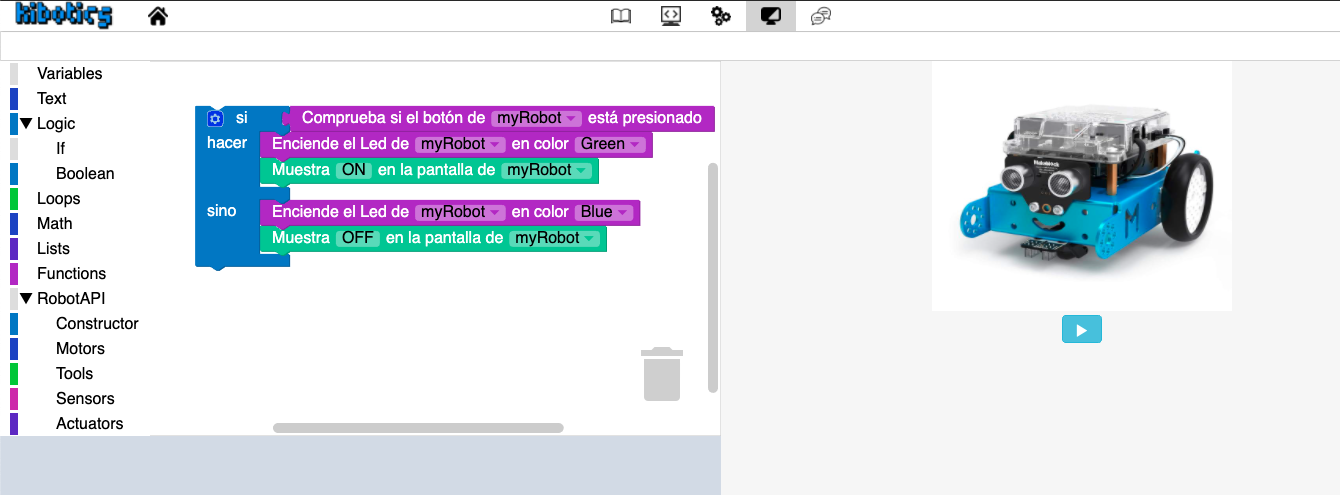
\includegraphics[width=0.9\textwidth]{images/editor_mbot.png}
  \caption{Editor Blockly para el Mbot }
  \label{figura:Editor Blockly para el Mbot }
\end{figure}
\\
Una vez que el usuario ha realizado el programa deseado y ha conectado el Mbot por USB a su ordenador, debe pulsar el botón azul que se muestra en la Figura 4.2 y, tras ello, se iniciará el proceso de envío.
\\
\\
En primer lugar, se abrirá una ventana que muestra los puertos del ordenador disponibles (Figura 4.3). Se debe seleccionar en el que se encuentra conectado el robot, que aparece nombrado como USB2.0Serial.
\\
\begin{figure}[h!]
  \centering
    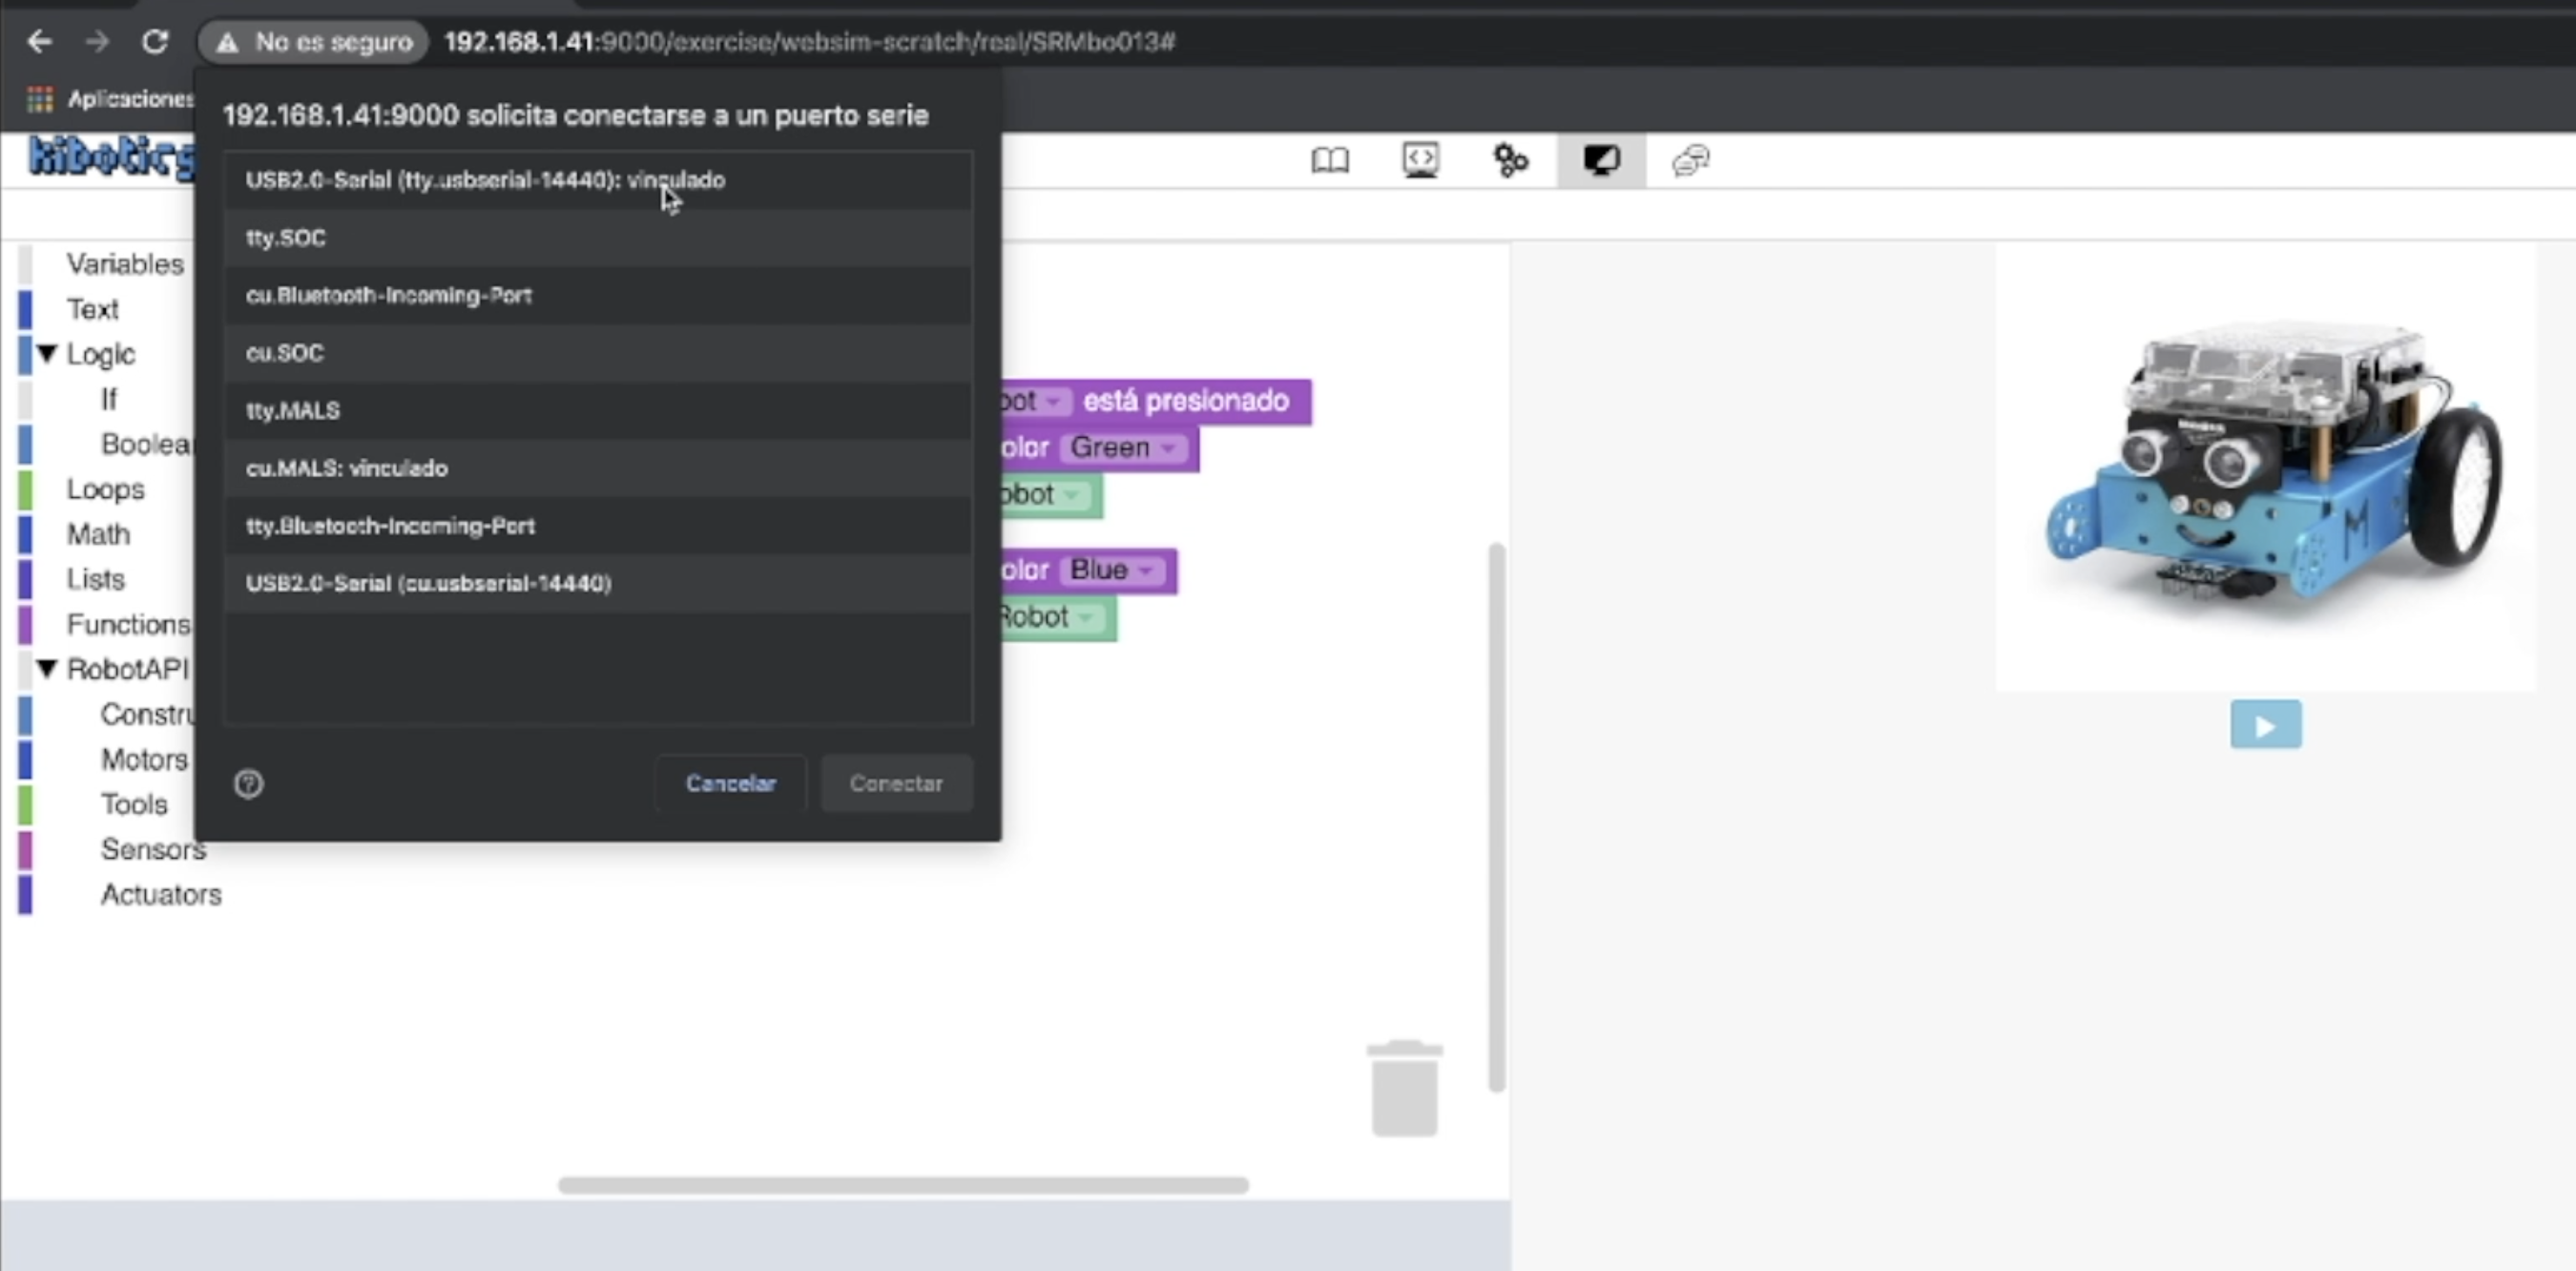
\includegraphics[width=0.9\textwidth]{images/seleccion_puerto.png}
  \caption{Selección puerto donde esta conectado el Mbot}
  \label{Selección puerto donde esta conectado el Mbot}
\end{figure}
\\
Tras seleccionar el puerto y pulsar “conectar”, el programa se cargará al Mbot. En el caso de haber cometido algún error durante el proceso, aparece un banner dando un aviso.

\section{Desarrollo realizado para la integración}

Este proceso descrito en la sección anterior es el que el usuario debería seguir para programar su robot, esto el como funciona a alto nivel, es decir, a ojos del usuario, pero por debajo se llevan a cabo una serie de acciones que permiten toda esta comunicación.
\\
\\
En la Figura 4.4 se muestra la infraestructura y las interacciones necesarias para conseguir cargar el programa al Mbot
\\
\begin{figure}[h!]
  \centering
    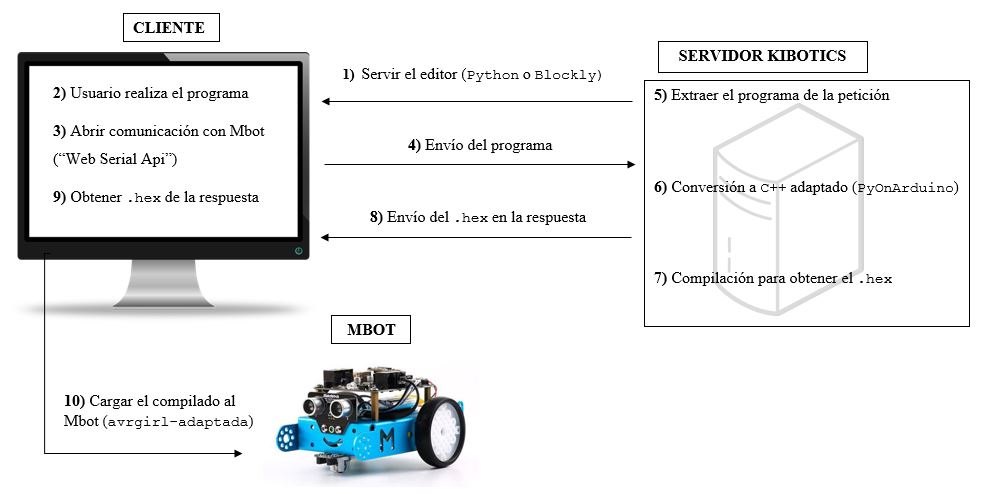
\includegraphics[width=1\textwidth]{images/infraestructura_mbot.png}
  \caption{Infraestructura seguida para la integración del Mbot}
  \label{Infraestructura seguida para la integración del Mbot}
\end{figure}
\\
\\
En los siguientes apartados se describen las fases principales que se deben seguir para enviar el programa al Mbot. Todo este proceso se inicia cuando el usuario ha realizado el ejercicio y ha pulsado “enviar”.

\subsection{Abrir una comunicación por el puerto serie}

El primer paso consiste en abrir una comunicación entre el navegador y el puerto serie donde está conectado el robot. Esta comunicación es posible gracias a “Web Serial Api”, que proporciona una Api al navegador; actualmente está disponible para el navegador Chrome.
Una vez que el usuario ha pulsado “enviar”, se procede a abrir la comunicación. Se abrirá el panel mencionado en el capítulo anterior (Figura 4.3) donde el usuario podrá conectarse al puerto donde se encuentra el Mbot y así poder iniciar la comunicación.
\\
\begin{lstlisting}[frame=single,breaklines=true, label=Abrir conexión con el Mbot por el puerto serie, caption=Abrir conexión con el Mbot por el puerto serie, captionpos=b]  % Inicia el bloque de código
   document.addEventListener('DOMContentLoaded', () => {

      document.getElementById('uploadMbot').addEventListener('click', clickConnect);

   });

   async function clickConnect() {
      progress.style.width = '0%';
      alertError.style.visibility = 'hidden';
      //-- Si el puerto serie estaba ya abierto, cerrarlo
      if (portPrev) {
         await disconnect();
      }
      await connect();
      activeProgress.style.visibility = 'visible';
      progress.style.width = '25%';
      if(document.getElementById('uploadMbot').value == 'python'){
          send_code_to_mbot()
      }else{
          convert_and_send_code_to_mbot();
      }

   }

   async function connect() {
      portPrev = await navigator.serial.requestPort();

      await portPrev.open({ baudrate: 115200 });

   }
   async function disconnect() {
       // -- Cerrar el puerto serie
      await portPrev.close();
      portPrev = null;
   }
\end{lstlisting}

\subsection{Enviar el programa para conversión}

Una vez abierta la comunicación de forma correcta, se procede a enviar el programa escrito al servidor mediante una petición GET y se introduce el programa como un query parameter en la URL. Para este envío se utiliza la función fetch() que está proporcionada por JavaScript.
\\
\begin{lstlisting}[frame=single,breaklines=true, label=Envio del programa desde el navegador al servidor, caption=Envio del programa desde el navegador al servidor, captionpos=b]
   function send_code_to_mbot() {
      var editor = ace.edit("ace");
      let code = editor.getValue();
      console.log(code);
      var enc = new TextEncoder();
      const message = {
         method: "GET"
       };
       url = '/get_python_to_arduino_binary?python_code=' + JSON.stringify(code);
       fetch(url, message)
             . . . . .
  
 }
\end{lstlisting}
Hay que tener en cuenta que si el programa está escrito en Blockly, debe convertirse previamente al lenguaje Python antes de enviarse, como puede verse en el fragmento 4.3.
\\
\begin{lstlisting}[frame=single,breaklines=true, label=Conversión de Blockly a Python, caption=Conversión de Blockly a Python, captionpos=b]
   var pythoncode = Blockly.Python.workspaceToCode(editor.ui);
\end{lstlisting}
El servidor recibe la petición del navegador y extrae el código del programa.
\\
\begin{lstlisting}[frame=single,breaklines=true, label=Extracción del programa en el servidor, caption=Extracción programa en el servidor, captionpos=b]
   def get_python_to_arduino_code_binary(request):
      . . . .
      python_code = json.loads(request.GET.get('python_code', None))
      . . . .

\end{lstlisting}

\subsection{Conversión del programa}

El programa extraído en el servidor es lenguaje Python, pero el Mbot, basado en Arduino como se mencionaba antes, no entiende este lenguaje. El lenguaje que usa Arduino es un C++ adaptado, por lo que se debe traducir desde Python. Esto es posible gracias a la librería PyOnArduino, la cual proporciona los mecanismos necesarios para esa traducción y conversión de un fichero.py (extensión para Python) a .ino (extensión para Arduino).
\\
\begin{lstlisting}[frame=single,breaklines=true, label=Traducción de lenguaje Python a Arduino, caption=Traducción de lenguaje Python a Arduino, captionpos=b]
   . . .    
    parsed_file = ast.parse(code)
    translator.robot = 'MBot'
    translator.robot_architecture = ''
    translator.vars.Variables()
    translator.vars.halduino_directory = py_to_arduino_path + 'HALduino/halduino'
    translator.TranslatorVisitor().visit(parsed_file)
    translator.create_setup()
    translator.variables_manager = translator.create_variables_manager(file=py_to_arduino_path + 'HALduino/variablesManager.ino')
    translator.create_output('output-file.ino')
    translator.create_makefile('MBot', py_to_arduino_path + 'makefiles/')
    . . .


\end{lstlisting}

\subsection{Compilado del programa}

Una vez extraído el código, se debe compilar para obtener el fichero .hex que contiene las instrucciones traducidas a hexadecimal entendidas por la microcontroladora. Esta compilación se lleva a cabo utilizando avrdude, una herramienta que permite la programación de chips AVR y que puede ser llamada por la línea de comandos.
\\
\begin{lstlisting}[frame=single,breaklines=true, label=Compilado y obtención del .hex, caption=Compilado y obtención del .hex, captionpos=b]
def create_mbot_binary():
    shutil.copyfile(os.path.join(settings.BASE_DIR, 'kibotics-drivers/mbot/avrdude'), './avrdude')
    shutil.copyfile(os.path.join(settings.BASE_DIR, 'kibotics-drivers/mbot/libftdi1.so'), './libftdi.so')
    shutil.copyfile(os.path.join(settings.BASE_DIR, 'kibotics-drivers/mbot/libreadline.so'), './libreadline.so.6')
    shutil.copyfile(os.path.join(settings.BASE_DIR, 'kibotics-drivers/mbot/avrdude.conf'), './avrdude.conf')
    shutil.copytree(os.path.join(settings.BASE_DIR, 'kibotics-drivers/mbot/arduino-1.8.10/'), 'arduino/')
    call(['make'])
    exercise_dir = './'
    # Extraemos el binario
    f_binary = open(exercise_dir + 'build-uno/output.hex', 'r')
    binary = f_binary.read()
    f_binary.close()
    return binary
\end{lstlisting}
Tras la compilación del programa, obtenemos el .hex, que será enviado como respuesta al navegador.
\\
\begin{lstlisting}[frame=single,breaklines=true, label=Respuesta a la petición que envió el navegador, caption=Respuesta a la petición que envió el navegador, captionpos=b]
    . . .
    binary = create_mbot_binary()

    response = HttpResponse(binary, content_type='text/plain')
    response['Content-Length'] = len(response.content)
    return response
\end{lstlisting}

\subsection{Respuesta de la petición}

De la respuesta enviada por el navegador con el programa realizado al servidor, se recibe una respuesta que contiene el programa compilado para poder enviárselo a la microcontroladora.
\\
\\
La función fetch(), mencionada anteriormente y la que permitía enviar una petición de lado del cliente, espera hasta recibir la respuesta, pudiendo extraer así el cuerpo de la respuesta, donde se encuentra la traducción del programa enviado.
\\
\begin{lstlisting}[frame=single,breaklines=true, label=Extracción del dato enviado en la respuesta, caption=Extracción del dato enviado en la respuesta, captionpos=b]
   fetch(url, message)
      .then(function(response) {
         if(response.ok){
            responseOk = true
         }else{
            responseOk = false
         }
           return response.text();
      })
      .then(function(data) {
        
         var dataBuffer = enc.encode(data);
           
      })
      .catch(function(err) {

         console.error(err);
       });

\end{lstlisting}

\subsection{Cargar compilado al robot}

Una vez extraído el código compilado, se procede a cargarlo en el robot. Avrgirl-arduino, una librería nodejs de código abierto, proporciona esa posibilidad de quemar el programa compilado a la microcontroladora, y es compatible con un gran número de placas (entre ellas ArduinoUno). Hemos utilizado esta librería adaptándola a nuestras necesidades para el proceso de carga.
\\
\begin{lstlisting}[frame=single,breaklines=true, label=Carga del compilado al Mbot, caption=Carga del compilado al Mbot, captionpos=b]
   . . . 
   
   .then(function(data) {

      if(responseOk){
         var dataBuffer = enc.encode(data);
         upload_to_mbot(dataBuffer)
         progress.style.width = '99%';
         alertError.style.visibility = 'hidden';
      }else{
         console.log("Fallo al compilar el programa")
         infoError.innerHTML = "Error"
         alertError.style.visibility = 'visible';
         activeProgress.style.visibility = 'hidden';
      }

   })
    . . . 
    
    function upload_to_mbot(dataBuffer){
       let avrgirl = new AvrgirlArduino({
          board: "uno"
       });

       avrgirl.flash(dataBuffer,(error) =>  {
          if (error) {
             console.error(error);
             portPrev = null;
             infoError.innerHTML = "Error!"
             alertError.style.visibility = 'visible';
             activeProgress.style.visibility = 'hidden';

          } else {
             console.info('done correctly.');
             portPrev = null
             alertError.style.visibility = 'hidden';
             activeProgress.style.visibility = 'hidden';
          }
      });
   }

\end{lstlisting}

\section{Resolución y experimentación}

En la explicación anterior no se ha mencionado en ningún momento para qué sistema operativo era compatible, y es aquí donde recae una de las principales ventajas de este desarrollo, pues al tratarse de una tecnología de lado del navegador proporciona compatibilidad para cualquier sistema operativo que disponga del navegador Chrome. Con ello, se consigue que esta herramienta sea multiplataforma.
\\
\\
Además, al no necesitar una instalación previa de dependencias o programas por parte del usuario, su usabilidad es más sencilla. Esto es muy importante de cara al uso de la plataforma, ya que, al estar orientada a alumnos de baja edad, es necesario que el proceso sea lo más simple posible.
\\
\\
La principal desventaja es que, actualmente, Web Serial Api está en fase de experimentación en Chrome, por lo que necesita ser activada con un proceso previo. Para ello, debemos escribir en el navegador Chrome “chrome://flags” y habilitar el flag “Experimental web Plataform features”.
\\ 
\\
Con el objetivo de verificar el funcionamiento se ha probado en diferentes sistemas operativos y ordenadores. Entre los que han sido probados se encuentran:
\begin{itemize}
	\item \textit{\textbf{Ubuntu 18.04}}.
	\item \textit{\textbf{Ubuntu 16.04}}
	\item \textit{\textbf{Windows 10}}.
	\item \textit{\textbf{Windows 7}}.
	\item \textit{\textbf{MacOs Catalina Versión 10.15.6}}.
	\item \textit{\textbf{MacOs Mojave Versión 10.14.6}}.
\end{itemize}

\chapter{Integracion Dron Tello en Kibotics}

En este capítulo se describe el desarrollo realizado para poder programar el dron Tello. A diferencia del Mbot, donde el proceso era similar para cualquier sistema operativo, en este caso el proceso va a variar.

\section{Características del dron Tello}

Tello es un mini dron distribuido por la empresa Ryze Technology (Figura 5.1). Debido a la facilidad de su uso, está destinado tanto a niños como a adultos que quieran aprender a utilizar drones. Puede alcanzar una velocidad de hasta 28 km/h, su radio de control abarca hasta los 100 metros y su señal de vídeo se transmite a una frecuencia de 2,4Ghz. Posee una unidad procesadora de Intel, un barómetro para controlar de altura, motores de tipo escobilla y una cámara de 720p. Además, sus hélices están protegidas y es resistente a las caídas.
\\
\\
Entre sus puntos fuertes destacan su gran estabilidad durante el vuelo y que utiliza un sistema de posicionamiento por visión (VPS). El sistema VPS utiliza un mínimo de dos cámaras para medir la distancia al suelo y la posición a la que se encuentra, compensando así los cambios en la posición que puedan darse (Castro, 2019).
\\
\begin{figure}[h!]
  \centering
    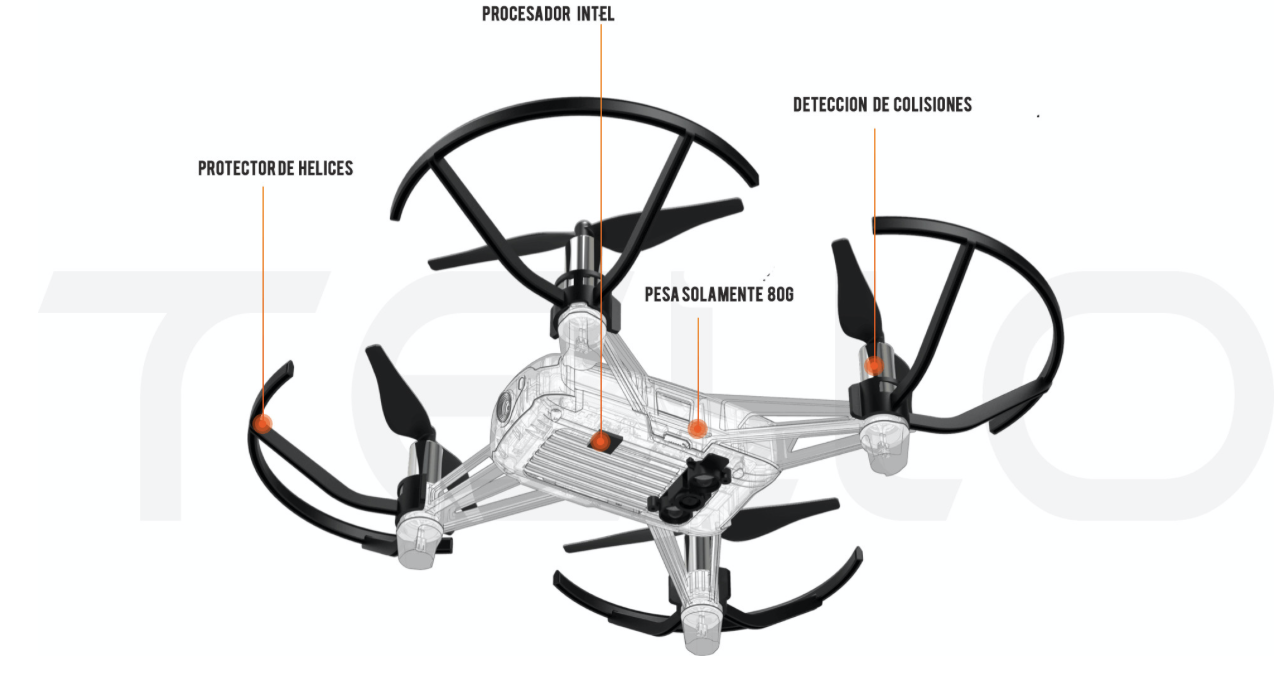
\includegraphics[width=0.9\textwidth]{images/partes_dron_tello.png}
  \caption{Esquema del dron Tello}
  \label{Esquema del dron Tello}
\end{figure}
\\

\section{Requisitos previos para su uso}

Para el Mbot no se requería ninguna instalación y, además, el proceso de envío del programa era el mismo para los diferentes sistemas operativos. En el caso del Tello, existen peculiaridades para los diferentes sistemas operativos al no tener control sobre la controladora que posee el robot y al necesitar un proxy intermediario
\\
\\
Para MacOs y Windows, es indispensable que el usuario tenga instalado Python en su versión 2.7 y los drivers necesarios para el uso del Tello. La empresa Dji-sdk posee un repositorio en GitHub (https://github.com/dji-sdk/Tello-Python) en el que se facilitan instaladores para su uso en los diferentes sistemas operativos.
\\
\\
En Linux, sin embargo, no es necesaria ninguna instalación previa para poder utilizar este dron. Esto es gracias a PyInstaller, una librería de Python, y a que el servidor de Kibotics se encuentra en una máquina Linux. En las próximas secciones se profundizará en este aspecto.

\section{Proceso de envío desde la plataforma Kibotics}

Al igual que el Mbot, en el dron Tello también existe la posibilidad de seleccionar la unidad dedicada a su programación en Python o en Blockly.
\\
\\
Una vez que el usuario ha desarrollado el programa, deberá pulsar el botón azul llamado “Ejecutar en Tello” (Figura 5.2) para iniciar el proceso de envío, que variará dependiendo del sistema operativo utilizado.
\\
\begin{figure}[h!]
  \centering
    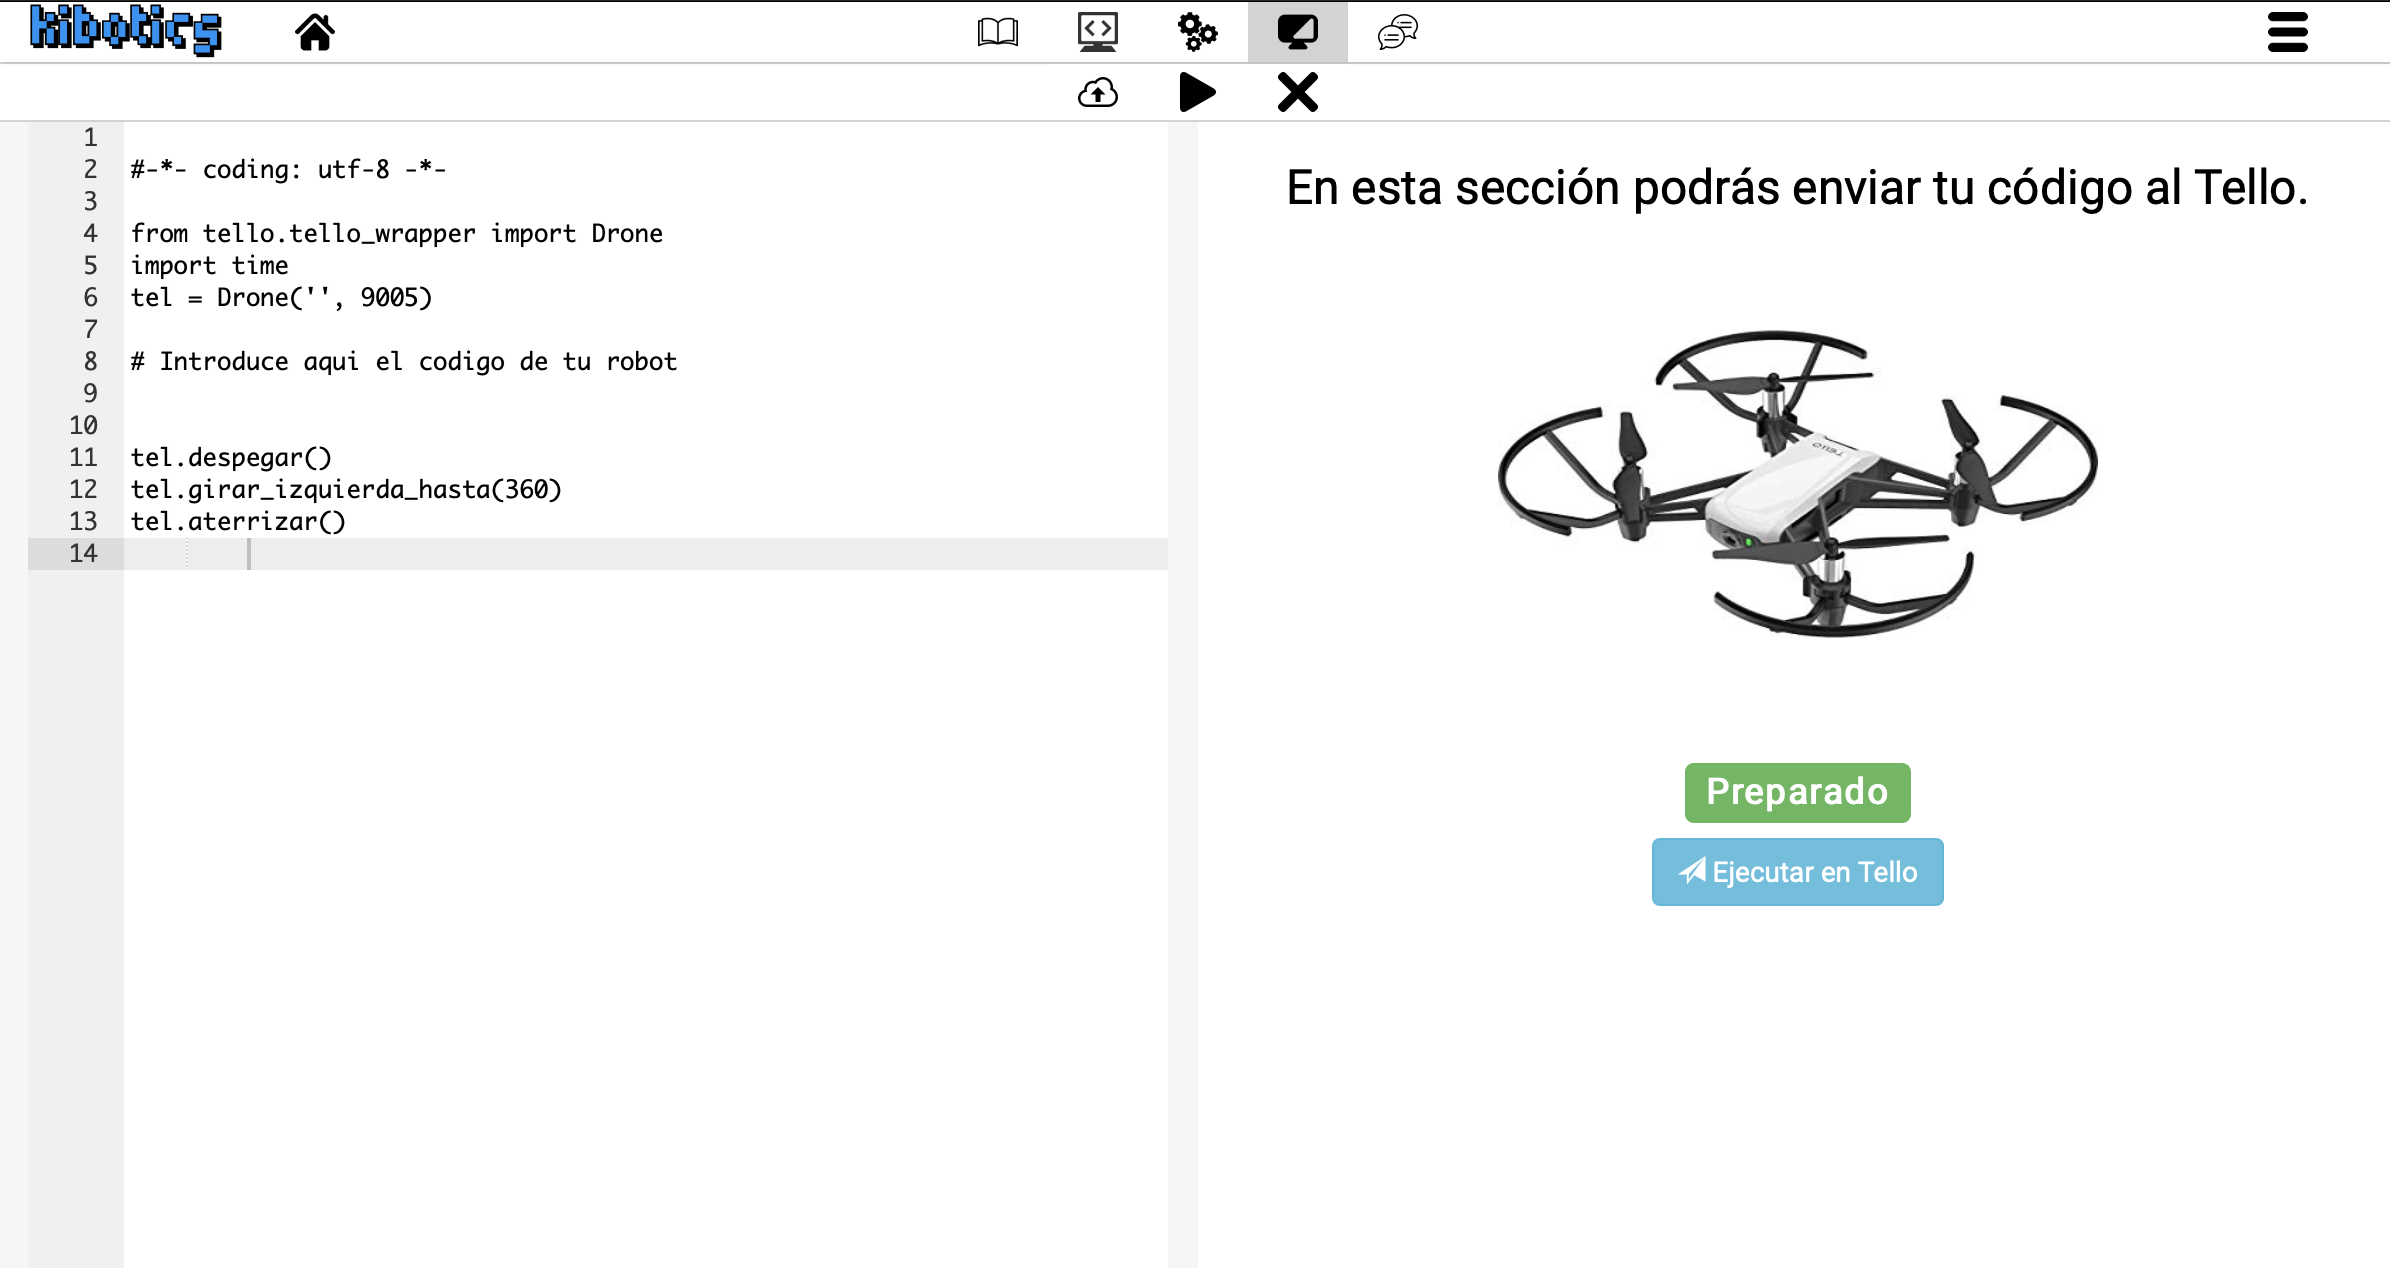
\includegraphics[width=0.9\textwidth]{images/editor_tello.png}
  \caption{Editor para programar el dron Tello en Python}
  \label{Editor para programar el dron Tello en Python}
\end{figure}
\\

\subsection{Proceso de envío para Linux}

\begin{enumerate}
	\item Se descargará un fichero ejecutable.
	\item Encender el dron Tello y conectarse a su punto de acceso WiFi (Figura 5.3).
	\\
		\begin{figure}[h!]
 			 \centering
    			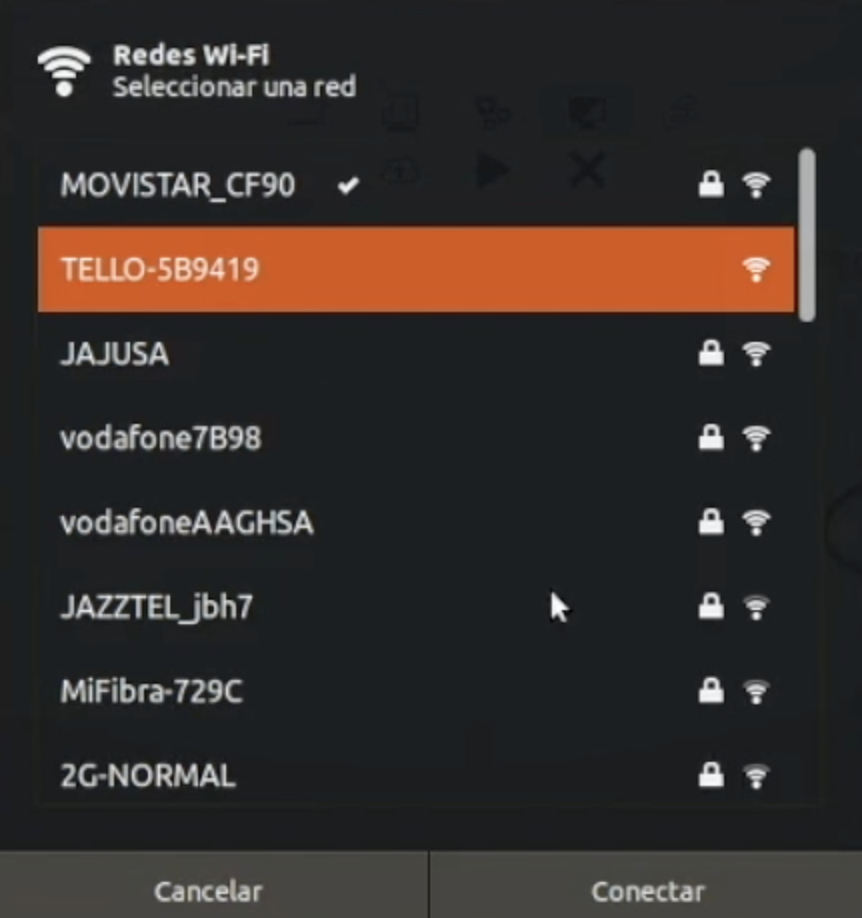
\includegraphics[width=0.4\textwidth]{images/seleccionar_wifi_tello.png}
  			\caption{Conectarse al punto de acceso WiFi emitido por el dron}
  			\label{Conectarse al punto de acceso WiFi emitido por el dron}
		\end{figure}
	\\
	\item Dirigirse al directorio donde se descargó el ejecutable, dar los permisos de ejecución y ejecutarlo con los comandos que se ven en el fragmento 5.1.
	\\
		\begin{lstlisting}[frame=single,breaklines=true, label=Comandos para ejecución del envío en Linux, caption=Comandos para ejecución del envío en Linux, , captionpos=b]
			chmod +x tello_code &&
			./tello_code

		\end{lstlisting}
	\item Una vez ejecutado, el programa se enviará al dron Tello.

\end{enumerate}
	
\subsection{Proceso de envío para Windows}

\begin{enumerate}
	\item Se descargará un fichero comprimido, que debe ser extraído.
	\item Encender el dron Tello y conectarse a su punto de acceso WiFi (Figura 5.3)
	\item Dirigirse al directorio donde se descomprimió el fichero (Figura 5.4)
	\\
		\begin{figure}[h!]
 			 \centering
    			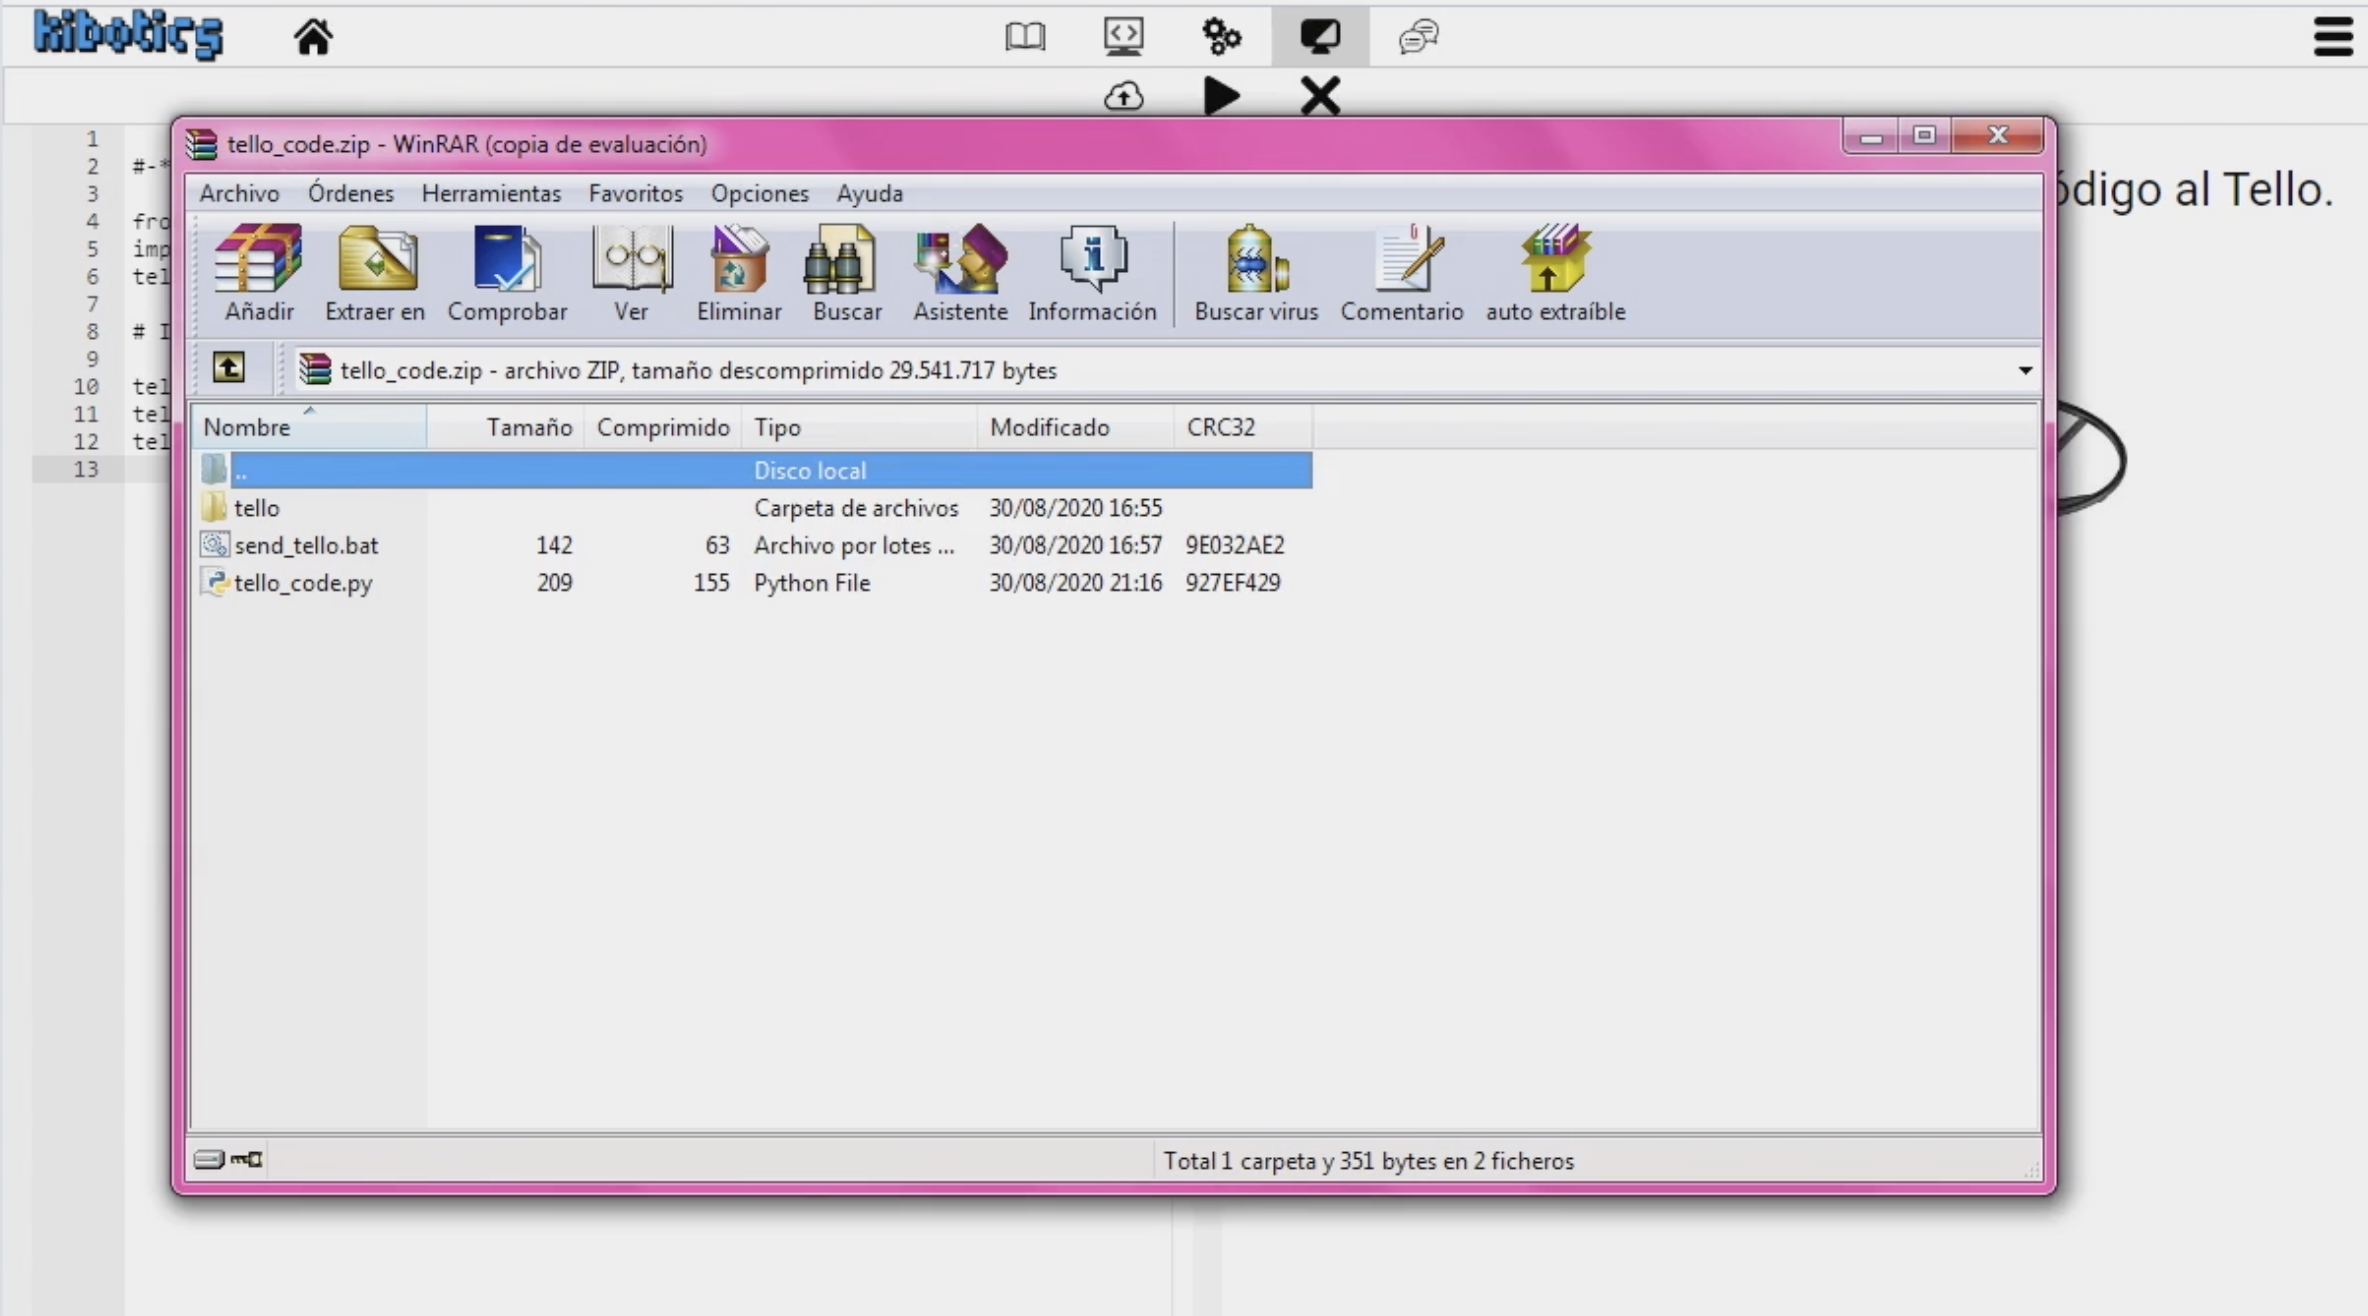
\includegraphics[width=1\textwidth]{images/descarga_windows_tello.png}
  			\caption{Descompresión en Windows}
  			\label{Descompresión en Windows}
		\end{figure}
	\\
	\item Haciendo doble “click” en el ejecutable send\_tello.bat, el programa será enviado al Tello.
\end{enumerate}

\subsection{Proceso de envío para MacOs}

\begin{enumerate}
	\item Se descargará un fichero comprimido, que debe ser extraído.
	\item Encender el dron Tello y conectarse a su punto de acceso WiFi (Figura 5.3).
	\item Dirigirse al directorio donde se descomprimió el fichero.
	\item Dentro del directorio se encuentra un archivo ejecutable llamado send\_code.sh, al que tendremos que dar permisos de ejecución y, posteriormente, ejecutarlo para enviar el programa al dron.
	\\
		\begin{lstlisting}[frame=single,breaklines=true, label=Comandos para ejecución del envío en MacOs, caption=Comandos para ejecución del envío en MacOs,  captionpos=b]
			chmod +x send_code.sh &&
			./send_code.sh
		\end{lstlisting}
\end{enumerate}

\section{Desarrollo realizado para la integración}

En la Figura 5.5, se muestra cuál es la arquitectura necesaria para conseguir el envío del programa al dron Tello.
\\
\begin{figure}[h!]
  \centering
    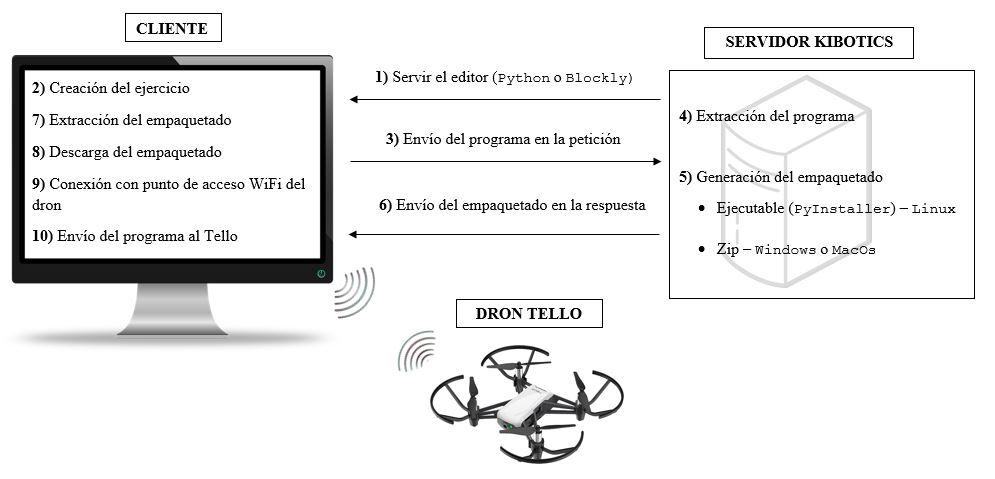
\includegraphics[width=1\textwidth]{images/infraestructura_tello.png}
  \caption{Arquitectura del desarrollo para el Tello}
  \label{Arquitectura del desarrollo para el Tello}
\end{figure}
\\
A continuación hablaremos en detalle sobre los pasos necesarios para conseguir la integración del Tello en Kibotics en los sistemas operativos Linux, Windows y MacOs.

\subsection{Envió del programa al servidor}

Este paso es similar al del Mbot. Una vez que el usuario ha realizado el programa y ha pulsado en el botón “Ejecutar en Tello” (Figura 5.2), se extrae del editor el código escrito y se envía desde el lado del navegador una petición al servidor de Kibotics con el programa realizado.
\\
\begin{lstlisting}[frame=single,breaklines=true, label=Envio del programa desde el navegador al servidor", caption=Envio del programa desde el navegador al servidor,captionpos=b]
   
   function send_code_tello() {
      var editor = ace.edit("ace");
      let code = editor.getValue();
      console.log(code);
      const message = {
         method: "GET"
       };
       var = url = '/get_code_to_tello?python_code=' + JSON.stringify(code);
       fetch(url, message)
             . . . . .
  }
\end{lstlisting}

Si el programa está escrito en Blockly, también es necesario convertirlo a lenguaje Python.
\\
\begin{lstlisting}[frame=single,breaklines=true, label=Convertir de Blockly a Python, caption=Convertir de Blockly a Python,captionpos=b]
   var pythoncode = Blockly.Python.workspaceToCode(editor.ui);
\end{lstlisting}

El servidor se encarga de extraer el programa enviado en la petición.
\\
\begin{lstlisting}[frame=single,breaklines=true, label=Extracción programa en el servidor, caption=Extracción programa en el servidor, captionpos=b]
   def get_code_to_tello(request):
      . . . .
      python_code = json.loads(request.GET.get('python_code', None))
      . . . .

\end{lstlisting}	

\subsection{Empaquetado del programa}

El dron Tello entiende el lenguaje Python, de manera que no es necesario convertirlo a otro lenguaje. Por lo tanto, una vez extraído el código se procede a su empaquetado, que será diferente en función del sistema operativo utilizado por el usuario.
\\
\begin{itemize}
	\item \textit{\textbf{Linux}}. Una vez extraído el código, se procede a realizar un ejecutable. Esto es posible gracias a una librería de Python llamada PyInstaller, un módulo que permite empaquetar ficheros Python, generando así un ejecutable e incluyendo dentro del propio ejecutable el intérprete de Python. PyInstaller no permite una compilación cruzada, es decir, si este empaquetado se realiza en una máquina Linux, el ejecutable solo podrá utilizarse en una máquina Linux. Debido a esto, la integración para el dron Tello varía según el sistema operativo; como el servidor de Kibotics está alojado en una máquina Linux, solo los usuarios de Linux se beneficiarán de esta utilidad.
\begin{lstlisting}[frame=single,breaklines=true, label=Creación ejecutable con PyInstaller, caption=Creación ejecutable con PyInstaller,  captionpos=b]
   def create_executable_with_pyinstaller(exercice_path):
    		      
   	call(". kibotics-drivers/tello/tello_env/bin/activate; pyinstaller -F --distpath " +
      	exercice_path + "dist --workpath " + exercice_path + "build --specpath " + exercice_path + " --clean " + exercice_path +
      	"tello_code.py", shell=True)
      . . . 
\end{lstlisting}
	Tras generar el ejecutable, se introduce en la respuesta que se enviará al navegador.
	\\
\begin{lstlisting}[frame=single,breaklines=true, label=Respuesta a la petición para Linux, caption=Respuesta a la petición para Linux,  captionpos=b]
   create_executable_with_pyinstaller(exercice_path)
   response = FileResponse(open(exercice_path + "dist/tello_code", 'rb'), content_type='application/octet-stream')
   shutil.rmtree(exercise_dir + "dist/")
   shutil.rmtree(exercise_dir + "build/")
   os.remove(exercise_dir + "tello_code.spec")
\end{lstlisting}
	
	\item \textit{\textbf{Windows y MacOs}}. El proceso es similar en ambos, pero diferente al caso anterior. Se empaqueta el programa con el directorio que engloba todas las librerías y las dependencias necesarias y que, además, contiene el ejecutable .bat (en Windows) o .sh (en MacOS) que se encargará del envío. La única diferencia entre ambos, es que al necesitar dependencias especificas por sistema operativo, se utilizan directorios diferentes en el empaquetado.
	\\
	\\
	Una vez realizado el empaquetado, se comprime en formato Zip y se introduce en la respuesta de la petición.
	\\
\begin{lstlisting}[frame=single,breaklines=true, label=Creación empaquetado y respuesta en Windows y MacOs, caption=Creación empaquetado y respuesta en Windows y MacOs,  captionpos=b]
   if operative_system == 'Mac':
        shutil.move(exercise_dir + "tello_code.py", os.getcwd() + "/kibotics-drivers/tello/MacOs")
        shutil.make_archive('output-tello-mac', 'zip', os.getcwd() + "/kibotics-drivers/tello/MacOs")
        os.remove(os.getcwd() + "/kibotics-drivers/tello/MacOs/tello_code.py")
        with open('output-tello-mac.zip', 'rb') as f:
            response = HttpResponse(f, content_type=guess_type('output-tello-mac.zip')[0])
            response['Content-Length'] = len(response.content)
            os.remove('output-tello-mac.zip')

    elif operative_system == 'Windows':
        shutil.move(exercise_dir + "tello_code.py", os.getcwd() + "/kibotics-drivers/tello/Windows")
        shutil.make_archive('output-tello-windows', 'zip', os.getcwd() + "/kibotics-drivers/tello/Windows")
        os.remove(os.getcwd() + "/kibotics-drivers/tello/Windows/tello_code.py")
        with open('output-tello-windows.zip', 'rb') as f:
            response = HttpResponse(f, content_type=guess_type('output-tello-windows.zip')[0])
            response['Content-Length'] = len(response.content)
            os.remove('output-tello-windows.zip')
\end{lstlisting}	

\end{itemize}

\subsection{Descarga del empaquetado y envío al Tello}

El navegador recibe la respuesta de la que se extraerá el ejecutable, en el caso de que se use una máquina Linux, o el comprimido, en el caso de usar Windows o MacOS. Posteriormente, se descarga en el ordenador.
\\
\begin{lstlisting}[frame=single,breaklines=true, label=Extracción empaquetado y descarga, caption=Extracción empaquetado y descarga,  captionpos=b]
   . . .
   
   var = url = '/get_code_to_tello?python_code=' + JSON.stringify(code);
   fetch(url, message)
      .then(response => {
         ld.style.display = "none";
         if (response.ok) {
            download_executable(response);
         } else {
            console.error("Bad Response");
         }
      })
     .catch(err => console.error(err));
   }
   
   function downloadExecutable(response) {
      response.blob().then(blob => {
         var down = document.createElement("down");
         document.body.appendChild(down);
         down.style = "display: none";
         url = window.URL.createObjectURL(blob);
         down.href = url;
         down.download = 'tello_code';
         down.click();
         window.URL.revokeObjectURL(url)
      })
   }
\end{lstlisting}
Una vez realizada la descarga, se puede realizar el envío al dron Tello, tal y como se explica en la sección 5.3.
\\
\\
El ejecutable que se utiliza en MacOS para el envío (send\_code.sh), con el objetivo de facilitar las instalaciones requeridas para el Tello, instalará todas las dependencias necesarias en el caso de que no se tengan en el ordenador.
\\
\begin{lstlisting}[frame=single,breaklines=true, label=Ejecutable de envio para MacOs, caption=Ejecutable de envio para MacOs,  captionpos=b]
   #!/bin/bash

   ######### Requirements #########

   env=~/.virtualenvs/tello-env
   if [ -d $env ];
   then
      source ~/.virtualenvs/tello-env/bin/activate
   else
      if ! type "pip" > /dev/null; then
         sudo easy_install pip
       fi
       if ! type "brew" > /dev/null; then
          /usr/bin/ruby -e "$(curl -fsSL https://raw.githubusercontent.com/Homebrew/install/master/install)"  
          brew update
       fi
       sudo brew install cmake
       sudo brew install boost
       sudo brew install boost-python
       sudo brew install ffmpeg
       sudo brew install tcl-tk
    
       mkdir ~/.virtualenvs
       pip install virtualenv
       virtualenv ~/.virtualenvs/tello-env --python=python2.7
       source ~/.virtualenvs/tello-env/bin/activate
       pip install SimpleWebSocketServer
       pip install numpy
       pip install matplotlib
       pip install opencv-python==3.1.0.1
   fi

   echo "################################"
   echo "### Sending program to tello ###"
   echo "################################"
   python tello_code.py
   echo "Program finished"
   deactivate
\end{lstlisting}

\section{Resolución y experimentación}

La tecnología utilizada en este caso es distinta a la del Mbot debido a las diferencias en las controladoras del robot; con Arduino, el control sobre ella es mayor, mientras que en la que utiliza el Tello no tenemos ningún control.
\\
\\
Otro aspecto importante es que para el envío del programa al Tello se necesita una pasarela, es decir, para poder comunicarnos con él necesitamos conectarnos al punto de acceso WiFi que emite el dron, por lo que no es posible un envío directo desde el navegador, algo que sí se podía hacer en el Mbot con Web Serial.
\\
\\
Por otro lado, la tecnología PyInstaller permite que el usuario interaccione con el dron sin necesidad de instalar previamente nada, y también simplifica el envío al lanzar el ejecutable descargado. El problema que surge es que, con la restricción de compilación cruzada, este proceso solo puede ser factible para Linux, ya que el servidor de Kibotics, que es el encargado de preparar el ejecutable, está alojado en una máquina Linux.
\\
\\
Para Windows y MacOs la situación cambia completamente. El usuario sí necesita tener instalado en su ordenador el intérprete Python2.7 y los drivers para poder usar el Tello, aunque en MacOs el ejecutable de envío será el que lo instale si el usuario no lo tiene, facilitando, por tanto, su uso. Además, el envío del programa no es tan directo, ya que en primer lugar hay que descomprimir el fichero descargado, que tiene las dependencias necesarias para el envío y, después, se lanza el ejecutable.
\\ 
\\
Para su experimentación se ha probado en diferentes sistemas operativos y ordenadores, verificando así el correcto funcionamiento de la integración. Entre los que han sido probados se encuentran:

\begin{itemize}
	\item \textit{\textbf{Ubuntu 16.04}}
	\item \textit{\textbf{Ubuntu 18.04}}.
	\item \textit{\textbf{Windows 10}}.
	\item \textit{\textbf{Windows 7}}.
	\item \textit{\textbf{MacOs Catalina Versión 10.15.6}}.
\end{itemize}

\chapter{GopiGo3}

\chapter{Conclusiones}
\subsection{Conclusiones}
\subsection{Líneas futuras}

\chapter{Bibliografía}

Báez, M.; Bongiovanni, P.; Castrillejo, D.; García, J. M.; Leal, D.; Levis, D.; Lugo, M. T.; Maguregui, C.; Ochoa, G.;  Peña-López, I.; Pisano, R.; Rabajoli, G.; Rivoir, A.; Sansberro, F.; Turner, N.; Vacca, A. M.; Vaillant, D. (2011). El modelo CEIBAL. Nuevas tendencias para el aprendizaje. Uruguay: CEIBAL - ANEP.
\\
\\
Bravo, F. Á.; Forero, A. (2012). La robótica como un recurso para facilitar el aprendizaje y desarrollo de competencias generales. \textit{Teoría de la Educación. Educación y Cultura en la Sociedad de la Información} 13(2): 120-139.
\\
\\
Castro, G. (6 de junio de 2019). DJI Tello, un minidron de juguete, programable con un procesador potentísimo. DronProfesional. Recuperado de https://dronprofesional.com/blog/dji-tello-un-minidron-de-juguete-programable-con-un-procesador-potentisimo/
\\
\\
Curso de iniciación a Python en Raspberry Pi. (2020). Recuperado 12 de septiembre de 2020, de Asociación Programo Ergo Sum website: https://www.programoergosum.com/cursos-online/raspberry-pi/244-iniciacion-a-python-en-raspberry-pi/que-es-python
\\
\\
González, J. J.; Jiménez, J. A. (2009). La robótica como herramienta para la educación en ciencias e ingeniería. \textit{IE Comunicaciones: Revista Iberoamericana de Informática Educativa} 10: 31-36.
\\
\\
Moreno, I.; Muñoz, L.; Serracín, J. R.; Quintero, J.; Patiño, K. P.; Quiel, J. (2012).\textit{ La robótica educativa, una herramienta para la enseñanza-aprendizaje de las ciencias y las tecnologías. Teoría de la Educación. Educación y Cultura en la Sociedad de la Información} 13(2): 74-90.
\\
\\
PYPL PopularitY of Programming Language index. (2020). Recuperado 15 de septiembre de 2020, de PYPL PopularitY of Programming Language website: http://pypl.github.io/PYPL.html
\\
\\
Quiroga, L. P. (2018). \textit{La robótica: otra forma de aprender. Revista Educación y Pensamiento} 25(25): 51-64
\\
\\
Robótica Educativa con Mbot. (2020). Recuperado 19 de septiembre de 2020, de Programo Ergo Sum website: https://www.programoergosum.com/cursos-online/robotica-educativa/249-robotica-educativa-con-mbot/que-es-mbot
\\
\\
REAL ACADEMIA ESPAÑOLA: \textit{Diccionario de la lengua española}, 23.ª ed., [versión 23.3 en línea]. <https://dle.rae.es> [12 de septiembre de 2020].
\\
\\
Ruiz-Velasco, E.; García, J. V.; Rosas, L. A. (2007). \textit{Robótica pedagógica virtual para la inteligencia colectiva}. México: Universidad Nacional Autónoma de México.
\\
\\
Salamanca, M. L.; Barrera, N.; Pérez, W. J. (2010). \textit{Uso de la robótica educativa como herramienta en los procesos de enseñanza}. Ingeniería Investigación y Desarrollo: I2+D 10(1): 15-23.
\\
\\
Shannon, R. E. (1998, diciembre 13-16). \textit{Introduction to the art and science of simulation}. In 1998 Winter Simulation Conference. Doi: 10.1109/WSC.1998.744890

\end{document}
